\documentclass[titlepage, a4paper,fleqn, oneside, 11pt]{article}

%inkluderer noen standarddefinisjoner
\input{/home/magnun/skole/latex/prefs.tex}
\usepackage{amsmath}
\begin{document}

\begin{figure}[h!]
\begin{center}
\scalebox{0.5}{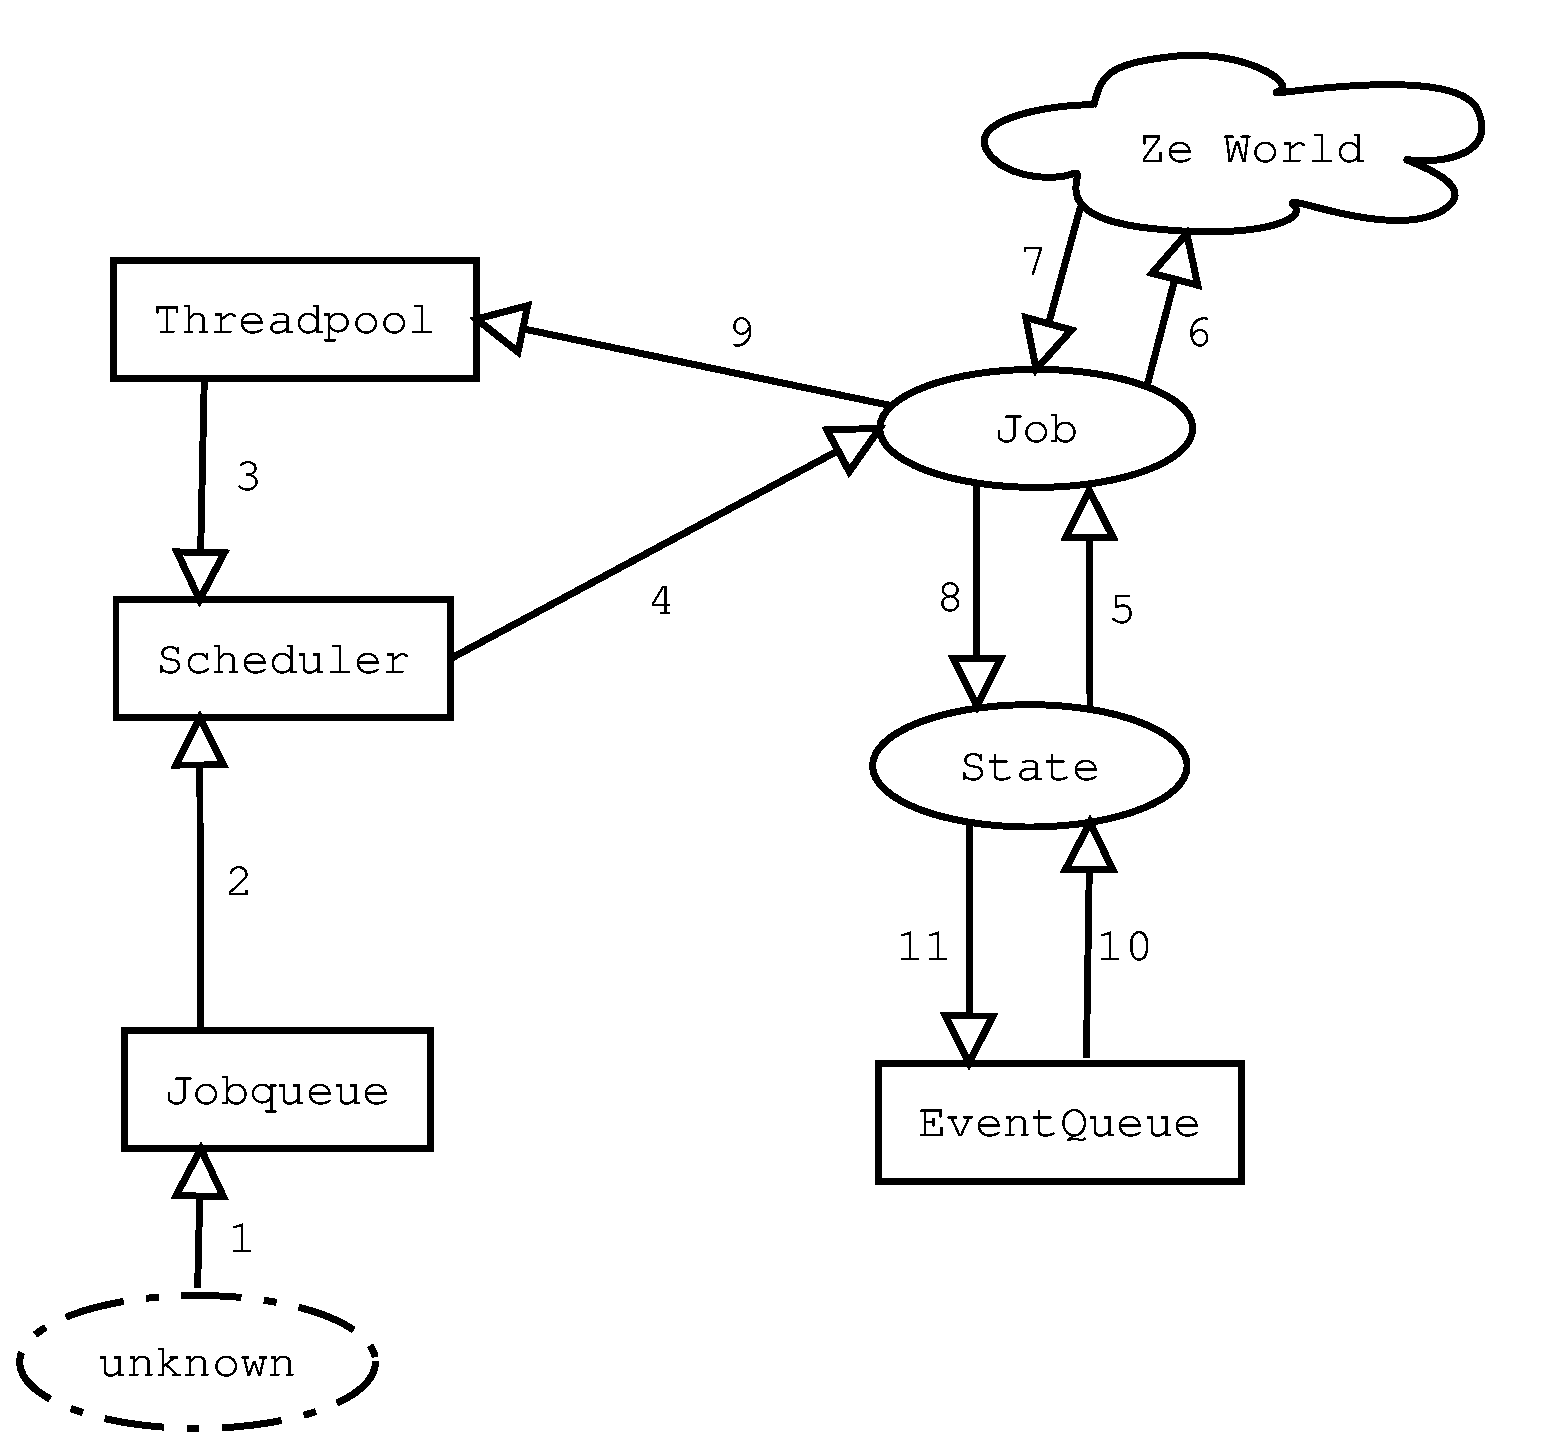
\includegraphics{abvehr.eps}}
\caption{}
\label{fig:foo}
\end{center}
\end{figure}


\newcounter{fig}
\begin{list}
{\arabic{fig}}{\usecounter{fig}\setlength{\rightmargin}{\leftmargin}}
\item Jobb blir plassert i jobbk�en. Er usikker p� hvordan dette skal gj�res.
\item Ledig tr�d
\item Henter jobb med h�yest prioritet
\item Jobben startes i tr�den
\item Jobben sjekker tilstand mot \emph{State}.
\item Sender foresp�rsel mot server/tjeneste
\item F�r respons fra server/tjeneste
\item Rapporterer resultat til \emph{State}
\item Jobben terminerer, og tr�den markeres som ledig
\item Dersom tilstanden er endret oppdateres \emph{EventQueue}
\item Sjekk tilstand i \emph{EventQueue}
\end{list}



\end{document}

%%% Local Variables: 
%%% mode: latex
%%% TeX-master: t
%%% End: 
